\documentclass{article}

% Drop neurips_2026.sty into this directory from the workshop template ZIP.
% Submission (anonymous) is the default; add [final] for camera-ready.
\usepackage{neurips_2026}

\usepackage[utf8]{inputenc}
\usepackage[T1]{fontenc}
\usepackage{hyperref}
\usepackage{url}
\usepackage{booktabs}
\usepackage{amsmath}
\usepackage{graphicx}
\usepackage{xcolor}

\title{Unexplained Variance Is Not Novel Signal:\\
Validating Interpretability-Derived Discovery in ECG Age Models}

% Anonymous for double-blind review.
\author{Anonymous Author(s)\\
Affiliation\\
Address\\
\texttt{email}}

\begin{document}

\maketitle

\begin{abstract}
Interpretability is increasingly used to argue that a model has discovered
something. A network predicts a clinical variable, its residual error is found
to be ``unexplained'' by standard measurements, attribution localises that
residual to an interpretable structure, and a discovery is claimed. We show this
inference is unsafe, and give a protocol that makes it testable.
Training a 12-lead ECG age regressor from scratch on PTB-XL, we find an
apparently significant association between its age-gap residual and myocardial
infarction ($+0.015$ AUC, significant after correction) that fails to replicate
across data splits and vanishes entirely when the set of already-measurable
quantities is expanded from 5 to 15 --- \emph{with no change to the model}. That
expansion quadrupled the variance attributable to existing knowledge, from
3.5\% to 14.6\%. The apparent magnitude of a discovery is therefore partly a
property of how thoroughly the analyst enumerated prior knowledge.
Applying the same discipline to attribution, we identify one claim that
survives: the model causally depends on atrial information that classical
P-wave measurement does not capture. It replicates across six independently
trained models in two cohorts on different continents and survives transferring
a model between them. We then turn the protocol on this claim as well, adding the
further atrial measurements cardiology reads --- terminal force, P-wave area,
notching --- and it narrows without closing, leaving three quarters of the age
gap unexplained. We report it as a falsifiable pointer, not a validated marker.
\end{abstract}

\section{Introduction}

Machine learning models now match domain experts across many scientific
settings, and appear to have learned regularities that humans have not
articulated. Interpretability offers a way to read those regularities back out,
and in clinical machine learning a standard argument has emerged: take a model's
residual error, show that it is not explained by established measurements,
localise it with attribution, and report a discovery.

The argument has a gap. Attribution answers \emph{where the model looked}. It is
structurally incapable of answering \emph{whether what it saw was already
known}. A model that has learned nothing more than ``a wider QRS complex means
an older patient'' --- a relationship cardiology has recorded for decades ---
produces exactly the same attribution figure as a model that found something
new. The two are indistinguishable at the level of the visualisation, and the
distinction is the entire question.

We study this on the ECG age gap: the difference between a model's predicted age
and a patient's chronological age, widely interpreted as a marker of
cardiovascular ageing. Predicting age from an ECG is an established task
\citep{attia2019age} and we claim no novelty for it; the model exists so that its
errors can be interrogated.

\paragraph{Contributions.}
\begin{enumerate}\itemsep2pt
\item A validation protocol separating rediscovery from discovery: regress the
candidate signal against enumerated prior knowledge, out of fold, adjusting for
covariates that mechanically induce correlation (\S\ref{sec:protocol}).
\item Null controls and a causal occlusion test for segment attribution on
physiological signals, addressing a confound we show can point attribution at
the wrong anatomical structure (\S\ref{sec:survives}).
\item An empirical demonstration that a statistically significant finding
dissolves under both, and a quantification of how much the conclusion depends on
the analyst rather than the data (\S\ref{sec:dissolves}).
\item One finding that survives every check, replicated in two cohorts, and then
subjected to the same enumeration test we use to dissolve the first --- including
a measurement we report as unmeasurable, with the noise floor that shows it
(\S\ref{sec:survives}).
\end{enumerate}

\section{Setup}
\label{sec:setup}

We use PTB-XL \citep{wagner2020ptbxl}: 21{,}799 clinical 12-lead ECGs, of which
21{,}373 remain after restricting to adults aged 18--89. Ages above 89 are
recorded as the sentinel value 300 for anonymisation; these are dropped rather
than clipped, since a fabricated age would corrupt both the regression target
and every residual computed from it. We use the dataset's own stratified folds
(17{,}090 / 2{,}132 / 2{,}151) and verify that no patient crosses a fold
boundary rather than assuming it.

The model is a 326{,}497-parameter 1D residual CNN trained from scratch, with no
pretrained weights anywhere in the pipeline. It reaches a test mean absolute
error of \textbf{7.32 years} ($R^2 = 0.694$), comparable to published ECG-age
models. It is deliberately small: an overfitted model's age gap is dominated by
memorisation noise, which would make every downstream analysis a study of
nothing.

One design choice changes conclusions and so belongs in the main text.
Classical intervals are measured at \textbf{500\,Hz} while the model consumes
100\,Hz input. At 100\,Hz one sample is 10\,ms, and on synthetic data with known
ground truth, QRS duration measured at 100\,Hz correlates with truth at
$r = 0.687$ against $r = 0.995$ at 500\,Hz. Since explained variance scales as
$r^2$, coarse measurement would leave roughly half of a \emph{genuinely known}
effect sitting in the residual, looking like a discovery.

\section{The protocol}
\label{sec:protocol}

Regress the candidate signal against everything already measurable and keep only
the remainder:
\[
\text{gap} \sim \text{demographics} \;\rightarrow\; R^2_{\text{base}},
\qquad
\text{gap} \sim \text{demographics} + \text{known} \;\rightarrow\; R^2_{\text{full}},
\]
\[
\text{attributable} = R^2_{\text{full}} - R^2_{\text{base}},
\qquad
\text{unexplained} = 1 - R^2_{\text{full}}.
\]
Only the unexplained part is eligible to be called a discovery candidate, and
even then it means ``we have not shown this is already known'', which is far
weaker than ``this is new''. Four components each prevent a specific failure.

\textbf{Demographic adjustment.} An age gap is mechanically anti-correlated with
age, because regression models pull towards the mean. Known measurements also
drift with age, so that shared dependence would be credited to them. In a
constructed case where an interval is a pure function of age and carries no
extra information, the unadjusted analysis credits it with over 60\% of the gap;
adjusted, under 10\%.

\textbf{Out-of-fold evaluation, grouped by patient.} In-sample $R^2$ rises with
model flexibility whether or not a relationship exists. An overfitting
\emph{baseline} is equally dangerous: several hundred trees fitted to two
demographic features on $\sim$100 recordings produced an out-of-fold $R^2$ of
$-31\%$, and subtracting a negative number inflated the attributable share to a
meaningless 84\%. We floor the baseline at zero --- a model that loses to the
mean explains nothing, not a negative amount.

\textbf{A rigid and a flexible explainer, both always reported.} A real but
non-linear dependence on a known measurement, missed by a linear fit, would sit
in the residual looking exactly like a discovery. Reporting both removes the
opportunity to select whichever number reads better.

\textbf{Measurements, not definitions.} On synthetic data we construct a T-wave
morphology change that leaves the true QT interval \emph{exactly} unchanged
($r = -0.001$ with the latent factor). \emph{Measured} QT nonetheless moves with
it ($r = +0.330$), because QT is measured by the tangent method, which reads the
slope of the T wave's descending limb. A change invisible to the \emph{definition}
of a known quantity can be partly visible to its \emph{measurement}. Only the
measurement can be regressed out, and only the measurement is what a clinician
has.

\paragraph{The error asymmetry.} Every weakness in this pipeline pushes the same
way. Noisy measurement, a thin known-feature set, an explainer too rigid to fit a
real relationship, and an overfitted model all \emph{shrink} the attributable
share and \emph{inflate} the unexplained residual. There is no corresponding
mechanism producing a false negative. A finding of ``fully explained'' is
therefore strong evidence, while ``largely unexplained'' is weak evidence --- and
much published inference in this area treats the latter as the stronger signal.

We validate the protocol against constructed ground truth in both directions: on
a synthetic cohort it correctly attributes a QRS-mediated age effect to known
features, and correctly leaves a morphology effect invisible to timing in the
residual (Appendix).

\section{Result 1: the discovery dissolves}
\label{sec:dissolves}

\begin{table}[t]
\centering
\caption{The same model and data analysed three ways, each stricter than the
last. Column A is a publishable positive finding. It survives neither a change
of split nor a fuller enumeration of prior knowledge. \textbf{Nothing about the
model changed between B and C} --- same architecture, seed, and test error.}
\label{tab:dissolve}
\small
\begin{tabular}{lccc}
\toprule
& A: 5 features, & B: 5 features, & C: \textbf{15 features}, \\
& own split & official folds & official folds \\
\midrule
Test MAE (years) & 7.53 & 7.32 & 7.32 \\
Attributable to known & 3.9\% & 3.5\% & \textbf{14.6\%} \\
Unexplained & 66.8\% & 75.8\% & \textbf{65.0\%} \\
$\Delta$AUC, myocardial infarction & \textbf{+0.015}$^{*}$ & +0.006 & \textbf{+0.001} \\
$\Delta$AUC, ST/T change & +0.004 & +0.017$^{*}$ & +0.001 \\
$\Delta$AUC, normal & +0.007$^{*}$ & +0.011$^{*}$ & +0.002 \\
\bottomrule
\end{tabular}
\vspace{2pt}
\footnotesize $^{*}$interval excludes zero after Bonferroni correction across
five diagnostic superclasses. Intervals are a paired percentile bootstrap
resampling patients, so recordings from one patient move together.
\end{table}

\begin{figure}[t]
\centering
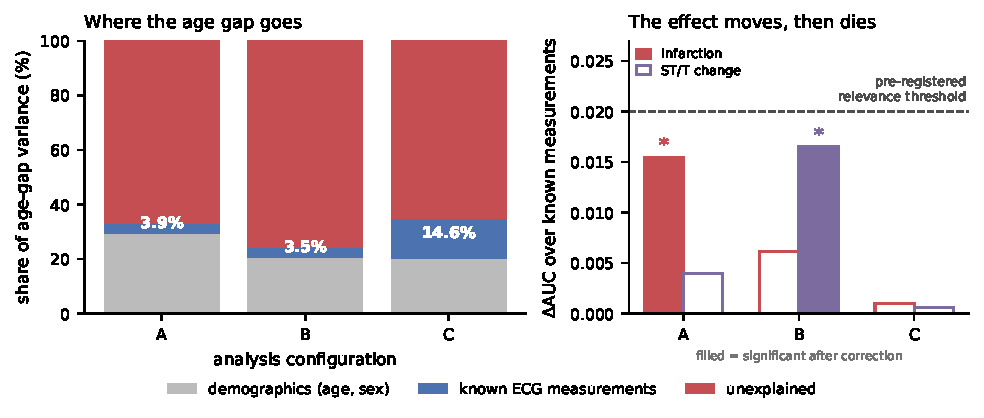
\includegraphics[width=\textwidth]{figures/fig1_dissolution.pdf}
\caption{The same model analysed three ways. \textbf{A}: five known features, our
own patient-level split. \textbf{B}: five features, the dataset's official folds.
\textbf{C}: fifteen features, official folds. Left: as prior knowledge is
enumerated more fully the attributable share (blue) quadruples. Right: the
myocardial-infarction association dies over the same three analyses, falling
below a relevance threshold fixed before any data was examined. \emph{The model
is identical in B and C.}}
\label{fig:dissolution}
\end{figure}

We ask whether the unexplained residual predicts cardiologist-assigned
diagnostic superclasses beyond the known measurements, comparing two logistic
classifiers differing by exactly one feature, on identical folds grouped by
patient. Table~\ref{tab:dissolve} reports three analyses of the same model.

Column A is a reportable positive result: after correction for testing five
superclasses, the unexplained age-gap residual improves myocardial infarction
detection. Reported alone it would read as a discovered biomarker. It does not
survive a change of data split (B), and it does not survive expanding the
known-feature set from five timing intervals to fifteen measurements including
amplitudes, electrical axes, ST deviation and R-wave progression (C).

Changing the split does not merely weaken the finding, it relocates it: in B the
infarction association falls below significance while ST/T change rises above it
at comparable magnitude. An analyst who ran B first would have reported a
different discovery with the same confidence, and neither survives C.

The mechanism is visible in the table. Between B and C the model is byte-for-byte
identical; only the analyst's enumeration of prior knowledge improved, and that
alone quadrupled the attributable share and drove the residual's incremental
value to $+0.001$ AUC. Under C no superclass retains a significant association.
We fixed a clinical-relevance threshold of 0.020 AUC before examining any data;
every effect in the table falls below it even where significant, and our
reporting code flags this automatically.

Two conclusions follow. For this model and dataset, the age gap carries no
clinically meaningful information beyond classical measurement. More generally,
\textbf{the apparent size of a discovery is a function of how thoroughly prior
knowledge was enumerated} --- a property of the analysis rather than the biology,
and invisible unless the known-feature set is deliberately varied.

\section{Result 2: a finding that survives}
\label{sec:survives}

Attribution requires its own controls. The QRS complex is by far the largest
deflection on an ECG, so gradients there are large regardless of what the model
learned. On synthetic data where the model's information was placed
\emph{entirely} in the T wave, density-based segment attribution nonetheless
pointed at the QRS; only comparison against an amplitude null exposed this. We
therefore compare every attribution profile against three nulls: per-segment
signal energy, an untrained model of the same architecture, and a model trained
on permuted labels.

The full four-segment profile against each null is given in
Appendix~\ref{app:nulls}; the shuffled-label control reached MAE 12.96 years
against a constant-prediction baseline of 13.21, confirming it learned nothing.

The model places more attribution on the \textbf{P wave} --- atrial
depolarisation --- than any null predicts: $+0.041$ above the amplitude null
(range $+0.033$ to $+0.050$), in 3/3 independently trained models, every interval
excluding zero, and unchanged when integration resolution is quadrupled. The
elevation localises to leads aVF, aVR, V1 and the limb leads, where P-wave
morphology is clinically assessed, and is \emph{negative} in V2--V3 where the P
wave is small and the QRS dominates. A uniform smear across all twelve leads
would have suggested an artefact.

\paragraph{Enumerating the atrial complex properly.} Result 1 says the size of a
discovery depends on how well prior knowledge was enumerated. That binds this
result too, so we applied it here rather than leaving it as future work.
Cardiology reads more from the P wave than duration, amplitude and PR interval:
we added \textbf{P terminal force in V1} (the Morris index of left atrial
abnormality), \textbf{P-wave area} and \textbf{P-wave notching}, all measured by
the same from-scratch signal processing. Table~\ref{tab:atrial} reports the
result. The attributable share rises from 2.5\% to 3.4\% --- a real movement,
positive in 8/8 explainer seeds when paired --- and \textbf{76\% of the age gap
remains unexplained}. The claim survives a fuller enumeration, weakened.

\begin{table}[t]
\centering
\caption{Our own surviving claim, tested against the enumeration the earlier
version of this paper listed as future work. Shares are means over eight
explainer seeds ($\pm$ SD); the delta is paired on seed. P-wave dispersion is
reported separately because it could not be measured, not because it was
skipped.}
\label{tab:atrial}
\small
\begin{tabular}{lcc}
\toprule
Known atrial measurements & Attributable & Unexplained \\
\midrule
P duration, P amplitude, PR interval & 2.5\% $\pm$ 0.4 & 77\% \\
\quad + terminal force, area, notching & \textbf{3.4\%} $\pm$ 0.3 & \textbf{76\%} \\
\midrule
\multicolumn{3}{l}{\footnotesize paired change $+0.8$ pp, positive in 8/8 seeds}\\
\bottomrule
\end{tabular}
\end{table}

Notably, P-wave \emph{area} is the strongest single atrial predictor of the age
gap ($r^2 = 0.026$), ahead of P amplitude (0.021): the three-measurement set used
previously was missing its best member. Notching contributes nothing, being
present in only 18\% of recordings. The
model's P-wave attention still tracks the classical measurements ($r = 0.47$ and
$r = 0.43$), so it is reading the atrial complex while extracting something those
numbers do not represent.

\paragraph{One measurement we could not make.} P-wave dispersion --- the spread of
P duration across the twelve leads --- needs P onset and offset found
independently in each lead rather than read from one window. We implemented it,
then measured its reliability against a cohort whose true dispersion is
\emph{zero} by construction, every lead being a fixed multiple of one shared P
component. There our per-lead delineation reports a median of \textbf{86\,ms}
where the truth is 0; on real PTB-XL it reports 80\,ms (SD 22\,ms). What we
measure on real data is thus indistinguishable from what we measure when the
answer is zero, and the noise floor alone exceeds the clinical range of the
quantity (20--50\,ms). We therefore report dispersion as \emph{unmeasurable
here}, not as a feature that failed to explain anything: an unreliable
measurement cannot shrink a residual, so its failure to do so is not evidence.

\paragraph{Occlusion: needed, not merely observed.} Attribution shows where a
model looks; a gradient can be large on a feature the prediction would survive
losing. We replace each segment with its per-lead isoelectric baseline in every
beat and compare against a \textbf{width-matched isoelectric control}: the same
number of samples blanked from electrically silent stretches. The control is
essential, because blanking any part of an ECG perturbs the input and a network
may degrade simply because its input became unfamiliar.

\begin{table}[t]
\centering
\caption{Causal occlusion ($\Delta$ MAE against a width-matched isoelectric
control) and external replication. Chapman-Shaoxing-Ningbo comprises 24{,}000
recordings from three Chinese hospitals, sharing no data with PTB-XL. Every
interval excludes zero.}
\label{tab:replication}
\small
\begin{tabular}{lcc@{\hspace{2em}}lcc}
\toprule
\multicolumn{3}{c}{\textbf{Occlusion}} & \multicolumn{3}{c}{\textbf{Chapman replication}} \\
\cmidrule(r){1-3}\cmidrule(l){4-6}
Segment & PTB-XL & Chapman & Arm & P attribution & P occlusion \\
\midrule
P wave & \textbf{+0.582} & \textbf{+1.043} & fresh, seed 0 & +0.049 & +0.65 \\
QRS & +7.348$^{\dagger}$ & +5.010$^{\dagger}$ & fresh, seed 1 & +0.079 & +1.15 \\
T wave & +0.617 & +1.006 & fresh, seed 2 & +0.049 & +1.33 \\
& & & \textbf{transfer} & +0.029 & +0.51 \\
\bottomrule
\end{tabular}
\vspace{2pt}
\footnotesize $^{\dagger}$inflated by distribution shift; see limitations.
\end{table}

Table~\ref{tab:replication} shows the P wave is causally required in 3/3 seeds on
PTB-XL, and that the whole result replicates on an independent cohort from three
Chinese hospitals with \emph{larger} effects ($+0.059$ attribution, $+1.043$
years occlusion). This occurs in an arrhythmia-enriched population where P waves
are \emph{harder} to detect (94.2\% of beats against 98.0\%), which is the
opposite of the pattern a cohort-specific artefact would produce.

The transfer arm separates two otherwise confounded things. Applied unchanged to
Chinese recordings, the PTB-XL model degrades substantially (MAE $7.32 \to 8.70$,
$R^2\ 0.694 \to 0.456$) --- a real domain shift --- yet the atrial dependence
persists with intervals excluding zero. \textbf{The model generalises poorly
while the finding generalises well}, which is evidence that the effect is a
property of ECGs rather than of one training set.

\begin{figure}[t]
\centering
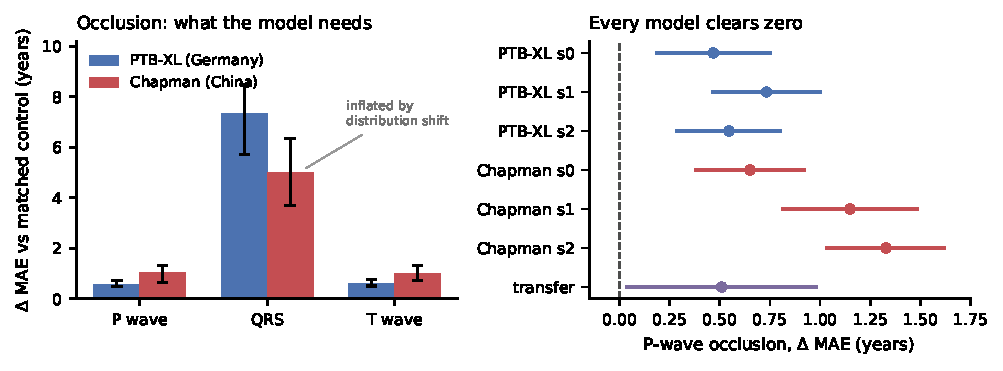
\includegraphics[width=\textwidth]{figures/fig2_occlusion.pdf}
\caption{Left: occlusion cost per segment against a width-matched isoelectric
control, both cohorts. Right: the P-wave effect for every model trained in this
study --- three per cohort plus the transferred model --- with 95\% intervals.
All seven clear zero.}
\label{fig:occlusion}
\end{figure}

\paragraph{The claim, stated at its actual strength.} The atrial complex carries
age information that this model causally depends on and that six classical
atrial measurements --- P duration, P amplitude, PR interval, terminal force,
area and notching --- do not capture. We stated the claim as falsifiable and then
ran the falsification ourselves rather than leaving it to a reader. It narrowed
the claim without closing it. This is a candidate that has survived one serious
attempt at dissolution by the same instrument that dissolved the finding in
Section~\ref{sec:dissolves}; the next attempt needs per-lead delineation good
enough to measure dispersion, which ours is not.

\section{Limitations and conclusion}

The QRS complex remains the dominant driver by roughly an order of magnitude per
sample ($+5.46$ against $+0.42$ years per 100 samples), so attribution's
\emph{relative} elevation of the P wave does not make it the model's principal
feature; and P and T are causally comparable, swapping order between seeds. The
QRS occlusion figure is inflated by distribution shift --- an ECG without QRS
complexes is far out of distribution, and one seed fell below the mean predictor
--- so the P-wave figure is the trustworthy one precisely because its
perturbation is gentler. The gross segment ranking correlates with the amplitude
null at $r = 0.929$; only the departures are the finding.

We have shown that six classical P-wave measurements do not capture the
dependence, not that none does. The candidate we could not test is dispersion,
and we can say precisely why: our noise floor on a zero-dispersion cohort is
86\,ms, above the whole clinical range of the measurement. Reporting it as a null
would have been reporting our own measurement error as a biological result.
Adding the three usable atrial measures to the fifteen-feature set of
Section~\ref{sec:dissolves} raises its attributable share from 14.5\% to 16.1\%,
so that known-feature set is incomplete too. Both cohorts are single-country, neither has
clinical outcome data, and our analysis covers adults 18--89 only. Occlusion
establishes that the model needs the information, not that the information is
biologically causal.

Interpretability tells you where a model looked. Deciding whether that
constitutes knowledge requires enumerating what was already known --- and the
answer is sensitive to how well that enumeration is done. We give a protocol,
demonstrate a finding dissolving under it, and one surviving.

\bibliographystyle{plainnat}
\begin{thebibliography}{9}
\small
\bibitem[Attia et al.(2019)]{attia2019age}
Z.~I. Attia et al.
\newblock Age and sex estimation using artificial intelligence from standard
12-lead ECGs.
\newblock \emph{Circulation: Arrhythmia and Electrophysiology}, 12(9), 2019.

\bibitem[Lima et al.(2021)]{lima2021ecgage}
E.~M. Lima et al.
\newblock Deep neural network-estimated electrocardiographic age as a mortality
predictor.
\newblock \emph{Nature Communications}, 12:5117, 2021.

\bibitem[Sundararajan et al.(2017)]{sundararajan2017ig}
M.~Sundararajan, A.~Taly, and Q.~Yan.
\newblock Axiomatic attribution for deep networks.
\newblock In \emph{ICML}, 2017.

\bibitem[Pan and Tompkins(1985)]{pan1985qrs}
J.~Pan and W.~J. Tompkins.
\newblock A real-time QRS detection algorithm.
\newblock \emph{IEEE Transactions on Biomedical Engineering}, 32(3):230--236, 1985.

\bibitem[Wagner et al.(2020)]{wagner2020ptbxl}
P.~Wagner et al.
\newblock PTB-XL, a large publicly available electrocardiography dataset.
\newblock \emph{Scientific Data}, 7:154, 2020.

\bibitem[Zheng et al.(2020)]{zheng2020chapman}
J.~Zheng et al.
\newblock A 12-lead electrocardiogram database for arrhythmia research covering
more than 10,000 patients.
\newblock \emph{Scientific Data}, 7:48, 2020.
\end{thebibliography}

\appendix
\section{Validating the protocol against constructed ground truth}
\label{app:synthetic}

We generate synthetic 12-lead ECGs with exactly known fiducial points and two
independent latent age offsets. One drives QRS widening and heart-rate change,
both classically measurable. The other drives T-wave \emph{skew}: a warped
raised-cosine that preserves the wave's onset, offset, duration and peak
amplitude exactly, so no timing interval can detect it by construction. Setting
either offset's variance to zero produces a cohort where the correct answer is
known.

The protocol behaves correctly in both directions. Where the age signal runs
entirely through QRS duration it recovers over 70\% of the explainable ceiling;
where it runs entirely through T-wave morphology it leaves over 50\% unexplained.
The ceiling matters: an age gap is the injected signal \emph{plus} the model's own
prediction error, and no measurement can explain a network's error, so demanding
100\% would be demanding an explanation for something absent.

\section{Signal-processing accuracy}
\label{app:signal}

All interval measurement is from-scratch classical signal processing with no
learned components: a Pan--Tompkins-style R-peak detector
\citep{pan1985qrs}, heuristic P- and T-wave delineation, and the tangent method
for T-wave offset.

Against constructed ground truth: R-peak detection reaches sensitivity 1.000 and
positive predictive value 1.000 with maximum error of one sampling interval at
both 100\,Hz and 500\,Hz. Measured intervals correlate with truth at
$r = 0.995$ (QRS duration), $0.985$ (PR) and $0.987$ (QT) at 500\,Hz.

On real recordings all measured intervals fall in published normal ranges in
both cohorts. P waves are detected in 98.0\% of PTB-XL beats and 94.2\% of
Chapman beats; the lower rate in the arrhythmia-enriched cohort is expected,
since atrial fibrillation genuinely lacks organised P waves.

\section{Two failures found only on real data}
\label{app:failures}

\paragraph{P-wave boundary search.} Our boundary search terminated at the first
sample falling below 20\% of P-wave height. A real P wave is roughly 0.1\,mV, so
that threshold is near the baseline noise floor. On clean synthetic data the
search terminated correctly; on PTB-XL it ran to the edge of the search window
in 22\% of beats, producing P waves wider than 200\,ms --- physiologically
impossible --- in 19.5\% of recordings, and PR intervals pinned at the window
ceiling in 16\%. Since PR is a known feature, this had been inflating the
unexplained residual. Fixed by requiring a sustained quiet run plus a
physiological width cap.

\paragraph{Silently zeroed gradients.} On Apple's Metal backend, Integrated
Gradients returned \emph{exactly zero} for 18 of 20 recordings at one batch size,
with no error raised and plausible-looking segment summaries. It was caught only
by checking the completeness axiom \citep{sundararajan2017ig}: relative error
0.90 against 0.004 on CPU. We now verify completeness on every call.

Both are recorded because they illustrate a general point: synthetic validation
is necessary but not sufficient, and an attribution method that violates its own
defining axiom can look entirely normal.

\section{Segment attribution against the three nulls}
\label{app:nulls}

\begin{table}[h]
\centering
\caption{Share of total absolute attribution per segment, PTB-XL. The elevation
of the P wave above every null is the finding; the gross ranking itself
correlates with the amplitude null at $r = 0.929$, so only the departures carry
information.}
\small
\begin{tabular}{lcccc}
\toprule
Segment & Trained & Amplitude & Untrained & Shuffled labels \\
\midrule
P wave & \textbf{0.119} & 0.086 & 0.081 & 0.056 \\
QRS complex & 0.341 & 0.320 & 0.358 & 0.578 \\
T wave & 0.178 & 0.225 & 0.213 & 0.110 \\
Isoelectric & 0.362 & 0.369 & 0.348 & 0.256 \\
\bottomrule
\end{tabular}
\end{table}

\section{Validating the extended atrial measurements}
\label{app:atrial}

Adding measurements to the known-feature set can only shrink a discovery claim,
so a measurement that is silently broken makes our own result look better than it
is. Each new measure is therefore validated in both directions - against a signal
whose answer is known, and against one whose answer is zero.

\paragraph{P terminal force.} Checked against constructed biphasic P waves with a
terminal negative run of known duration and depth; the index equals their product
and orders recordings by depth as the Morris criterion requires. A P wave ending
above baseline returns exactly zero, which is an observation rather than a
missing value.

\paragraph{P-wave area.} Its absolute value is not known a priori, because each
lead scales the P component by its own coefficient. We instead check the
invariances that would break if the integration window or the baseline were
wrong: doubling P amplitude doubles the area, and widening the P wave by 40\%
widens the area by 40\%. We also verify area is not a deterministic function of
duration and amplitude, since a measure recoverable from two we already had
would add nothing.

\paragraph{P-wave notching.} The false-positive control is the important one. An
unsmoothed P wave has many local maxima, so a naive peak count reports every
recording as notched and would fabricate an explanation for the residual. Our
detector returns exactly zero on smooth raised-cosine P waves and on ten noise
realisations of them, detects constructed bifid waves, and reports a notch depth
that grows monotonically as the two humps separate.

\paragraph{P-wave dispersion, and why it is absent from Table~\ref{tab:atrial}.}
The synthetic cohort's twelve leads are exact linear projections of three shared
components, so all leads share one P onset and offset and true dispersion is
identically zero. We assert that premise in the test suite rather than trusting
it, since it is what the noise-floor argument rests on. Measured on that cohort
under its normal interference levels, our per-lead delineation reports a median
dispersion of 86\,ms where the truth is 0\,ms. The real-data median is 80\,ms.
The measurement is therefore uninformative here: it returns approximately the
same value whether or not any dispersion exists. Note that this is a statement
about our pipeline, not about the clinical quantity - P-wave dispersion is
measurable with delineation validated against annotated per-lead boundaries,
which is exactly what this project's from-scratch, no-pretrained-components
constraint excludes.

\section{Inference procedure for the diagnostic link}
\label{app:inference}

For each superclass we fit two $\ell_2$-regularised logistic classifiers on
identical patient-grouped folds, differing by exactly one feature: the
unexplained age-gap residual. Both are given age and sex, so the comparison is
incremental over demographics as well as over the known measurements. We pool
out-of-fold predictions before scoring, rather than averaging per-fold AUCs,
because superclass prevalence varies across folds.

Confidence intervals come from a paired percentile bootstrap over the pooled
out-of-fold predictions: each replicate resamples \emph{patients} with
replacement and carries all of a patient's recordings together, then recomputes
both AUCs and their difference on the same resample. Resampling patients rather
than recordings matters because PTB-XL contains repeated recordings of the same
individual, and treating them as independent would understate the variance. The
paired construction matters because the two classifiers are scored on identical
data and their AUCs are strongly correlated; the difference is far better
determined than either endpoint. We correct for testing five superclasses by
widening each interval to the Bonferroni-adjusted level.

We record an earlier error here because it bears on how such intervals should be
read. A previous version of this analysis formed its interval from percentiles
of the five \emph{per-fold} deltas. That is not a confidence interval. With five
folds, the Bonferroni-corrected lower tail is simply the minimum of five
numbers, so the significance flag had silently degraded into ``every fold came
out positive'' --- a sign test with no stated error rate --- and fold estimates
are not independent draws in any case, since their training sets overlap.

Correcting it changed two entries of Table~\ref{tab:dissolve}, in opposite
directions: the residual's association with the \emph{normal} class under
configuration C lost significance, and its association with ST/T change under
configuration B gained it. The old rule was not conservative or liberal but
simply uncalibrated, and a rule that errs in both directions cannot be diagnosed
by checking whether its answers look reasonable. We note that the paper's own
thesis applies to the paper: the apparent strength of a finding depends on
analysis choices that stay invisible until deliberately varied, and the
significance machinery is as susceptible to this as the enumeration of prior
knowledge is.

\section{Reproducibility}
\label{app:repro}

Both datasets are public and CC BY 4.0. The full pipeline runs end to end on
procedurally generated data with no downloads required, and the test suite
(366 tests) verifies every ground-truth claim above. Model parameters are
bit-for-bit determined by the random seed, which is also how the
no-pretrained-weights claim is checked. Attribution runs on CPU by default for
the reason in Appendix~\ref{app:failures}.

\section*{Responsible use statement}

This work studies claims that machine-learning models have discovered new
clinical knowledge, and argues that such claims are systematically easier to
make than to justify. The societal risk is direct: an unvalidated
``AI-discovered biomarker'' can redirect research funding and clinical attention,
and a claim that does not replicate consumes those resources without benefit. We
demonstrate that failure mode concretely, in our own analysis, where an
apparently significant association did not survive a change of data split or a
fuller enumeration of existing knowledge.

The risk our own positive result carries is that it be over-read. We report a
model's causal dependence on atrial information not captured by six classical
P-wave measurements. This is a pointer for investigation, \textbf{not a clinical
finding}: it establishes neither biological causation, nor clinical utility, nor
that no existing measurement captures the signal, and it must not inform patient
care. Our mitigations are to state the claim's exact scope in the main text
rather than an appendix, to report effect sizes alongside significance against a
threshold fixed before analysis, and to release code sufficient to reproduce or
refute every number.

Both datasets are fully de-identified, publicly released under CC BY 4.0, and
used within their licence terms; no new patient data was collected. Both cohorts
are single-country and the analysis is restricted to adults aged 18--89, so
nothing here should be assumed to transfer to paediatric populations or to other
health systems.

\end{document}
